%
% string matching writeup...
%

\documentclass{llncs}
\pagestyle{empty}
\usepackage{makeidx}  % allows for indexgeneration
%
\usepackage[dvips]{graphicx}    % needed for including graphics e.g. EPS, PS
\usepackage{epsfig}
\usepackage{url}
\usepackage{pseudocode}
\usepackage{comment}
\usepackage{authblk}
\usepackage{color}
\usepackage{newalg}
\usepackage{subfigure}

\begin{document}
\renewcommand{\labelenumi}{(\Alph{enumi})}
\renewcommand{\labelenumii}{(\alph{enumii})}

\frontmatter          % for the preliminaries
%
\pagestyle{headings}  % switches on printing of running heads

\mainmatter              % start of the contributions
%
\title{Bridging the gap: improving local multiple alignment with gapped extension.}
%
\titlerunning{procrastination for local multiple alignment}  % abbreviated title (for running head)
%                                     also used for the TOC unless
%                                     \toctitle is used
\author{...}

%\institute{ 
%Algorithms and Genetics Group, Dept. of Computer Science, Technical Univ. of Catalonia, Barcelona, Spain\\
%\email{treangen@lsi.upc.edu},\\
%}
%
\authorrunning{<Quijote> et al.}   % abbreviated author list (for running head)

\maketitle


\begin{abstract}
The identification of homologous DNA via sequence alignment is a basic building block in comparative genomics.  We present a method for accurately and sensitively identifying homologous DNA sequence in multiple genomes. Our method is based around an efficient heuristic for local multiple alignment, featuring a novel method for gapped extensions. In practice, we are able to sensitively identify conserved, potentially repetitive, regions in one or more DNA sequences.  The GPL implementation of our algorithm in C++ is
called \texttt{procrastAligner} and is freely available from
\url{http://gel.ahabs.wisc.edu/procrastination}
\end{abstract}




\section{ Introduction }

A central task in comparative genomics is being able to accurately identify all homologous positions in one or more DNA sequences. Local sequence alignment methods~\cite{blast,...} are considered to be the main tool for this task. The focus was on pairwise homology relationships, that is, detecting all possible pairs of homologous regions in the input sequence(s) via local pairwise alignment.  Local pairwise alignments can then be expanded to multiple relationships by grouping all pairwise homologous regions into groups(blocks,piles)~\cite{...}. Even so, multiple alignment methods based around pairwise local alignment experience several difficulties when attempting to create multiple relationships from pairwise. Local pairwise alignment has been demonstrated to be less accurate than local multple alignment~\cite{...}, especially when dealing with many DNA sequences. Also, highly repetitive regions in the input sequences can cause problems in efficiency, as they must conduct $O(n^{2})$ pairwise comparisons for each of the repeated regions.  Finally, methods based around pairwise local alignments often experience difficultly resolving inconsistencies when attempting to glue or merge all pairwise relationships. Highly repetitive ALU repeats and IS elements in microbes are just two common examples of the overwhelming abundance of repetitive sequence in genomes.

Local multiple alignment offers an alternative approach which inherently avoids some of the aforementioned difficulties. For example, instead of aligning all possible pairs of the repeat, a single local multiple alignment can be constructed. Local multiple alignments have also been shown to be more accurate pairwise local alignment when dealing with many input sequences~\cite{cite a paper which shows multiple alignment is more accurate than pairwise alignment}. Local multiple alignment also offers a better approach for resolving and merge boundaries of homology between all pairwise relationships.  As such, local multiple alignments identify the basic repeating units in one or
more sequences and can serve as a basis for downstream analysis
tasks such as multiple genome alignment~\cite{ref-mauve,ref-mga,ref-mgcat,ref-deweyReview}, global
alignment with repeats~\cite{ref-otherSammethPaper,ref-aba}, or
repeat classification and analysis~\cite{ref-piler}. Say something about how repeats are important, abudundant, and that they need to be accurately identified.

FIXME.. what am I trying to say here??

Due to the cost of alignment in multiple sequences grows exponentially with respect to the number of sequences, we must find clever ways to perform and limit the amount of gapped alignment via dynamic programming that is performed. Gapped alignments arise when trying to extend seeds to fully capture surrounding sequence homology. Our aim is to bridge this gap in efficiency by presenting a novel method for gapped extension for sensitive local multiple alignment.

%related methods

Related methods to our approach include TBA/MULTIZ, RepeatScout(well not really...), ABA(are you sure?),  and the Eulerian path approach to local multiple alignment.

FIXME.. this needs to be rewritten!

TBA/MULTIZ finds a set of local multple alignments and projects them onto a reference sequence in order to build whole genome comparisons. However, TBA relies on multiz to build multiple relationships of sequence homology from local pairwise relationships using multiz. ABA ... Perhaps the most related approach is Eulerian path approach to local multiple alignment...

CONSENSUS based approaches to local multiple alignment. Euler, RepeatScout. Has the advantage that it is relatively easy to find and construct local multiple alignments using the pairwise local alignment searches for the consensus sequences. Drawbacks?? 

looks like we are in a battle with RepeatScout and Eulerian path approach?

%



%need for a new approach
%To date~\cite{gold}, there are over 500 completed whole genomes in such databases, and in the next few years this number is %expected to reach nearly 3000. To cope with such increases in data volume, corresponding advances in computational methods are %necessary; thus we present an efficient heuristic for local multiple alignment. Our method is based around an efficient %heuristic for local multiple alignment, featuring a novel method for gapped extensions.
\label{sec:overview}
\section{Definitions and Notation}

Given a sequence $\mathcal{S}=s_1, s_2,\dots, s_N$ of length $N$
defined over an alphabet $\{A,C,G,T\}$, our goal is to identify all homologous
local multiple alignments on subsequences of $\mathcal{S}$. We denote
an ungapped alignment, or match, among subsequences in $\mathcal{S}$
as an object $M$.  We refer the number of regions in $\mathcal{S}$
matched by a given match $M_i \in \mathbf{M}$ as the
\textit{multiplicity} of $M_i$, denoted as $|M_i|$. We refer to each
matching region of $M_i$ as a \textit{component} of $M_i$. Note that
$|M_i| \geq 2~\forall~M \in \mathbf{M}$. We will refer to a match $M$ with $M_i>1$ as a multi-match. 
When aligning DNA sequences, matches may occur on the forward or reverse complement strands. To account for
this phenomenon we add an orientation value to each matching region
where 1 indicates a forward strand match and -1 for reverse.

Our algorithm has an important limitation on the matches in
$\mathbf{M}$: no two matches $M_i$ and $M_j$ may have the same
left-end coordinate, e.g. $M_i.L_x \neq M_j.L_y~\forall~i, j, x, y$
except for the identity case when $i=j$ and $x=y$.  This constraint
has been referred to by others as \textit{consistency} and
\textit{transitivity}~\cite{ref-transitivity} of matches.  However, seed matches may overlap.

We denote a gapped alignment over an alphabet $\{A,C,G,T,-\}$ as $A$. FIXME: what more do we need to say about gapped alignments?

\section{A heuristic for local multiple alignment}

Our heuristic for local multiple alignment
can be divided into five independent steps:
(1) detection of multi-matches using palindromic spaced seeds
(2) prioritized chaining of all multi-matches
(3) gapped extension of all chains
(4) estimation of homologous sequence boundaries using random walk statistics
(5) unalignment of all non-homologous sequence in local multiple alignment

\begin{figure}[t]
\begin{center}
\subfigure[Visual representation of our algorithm]{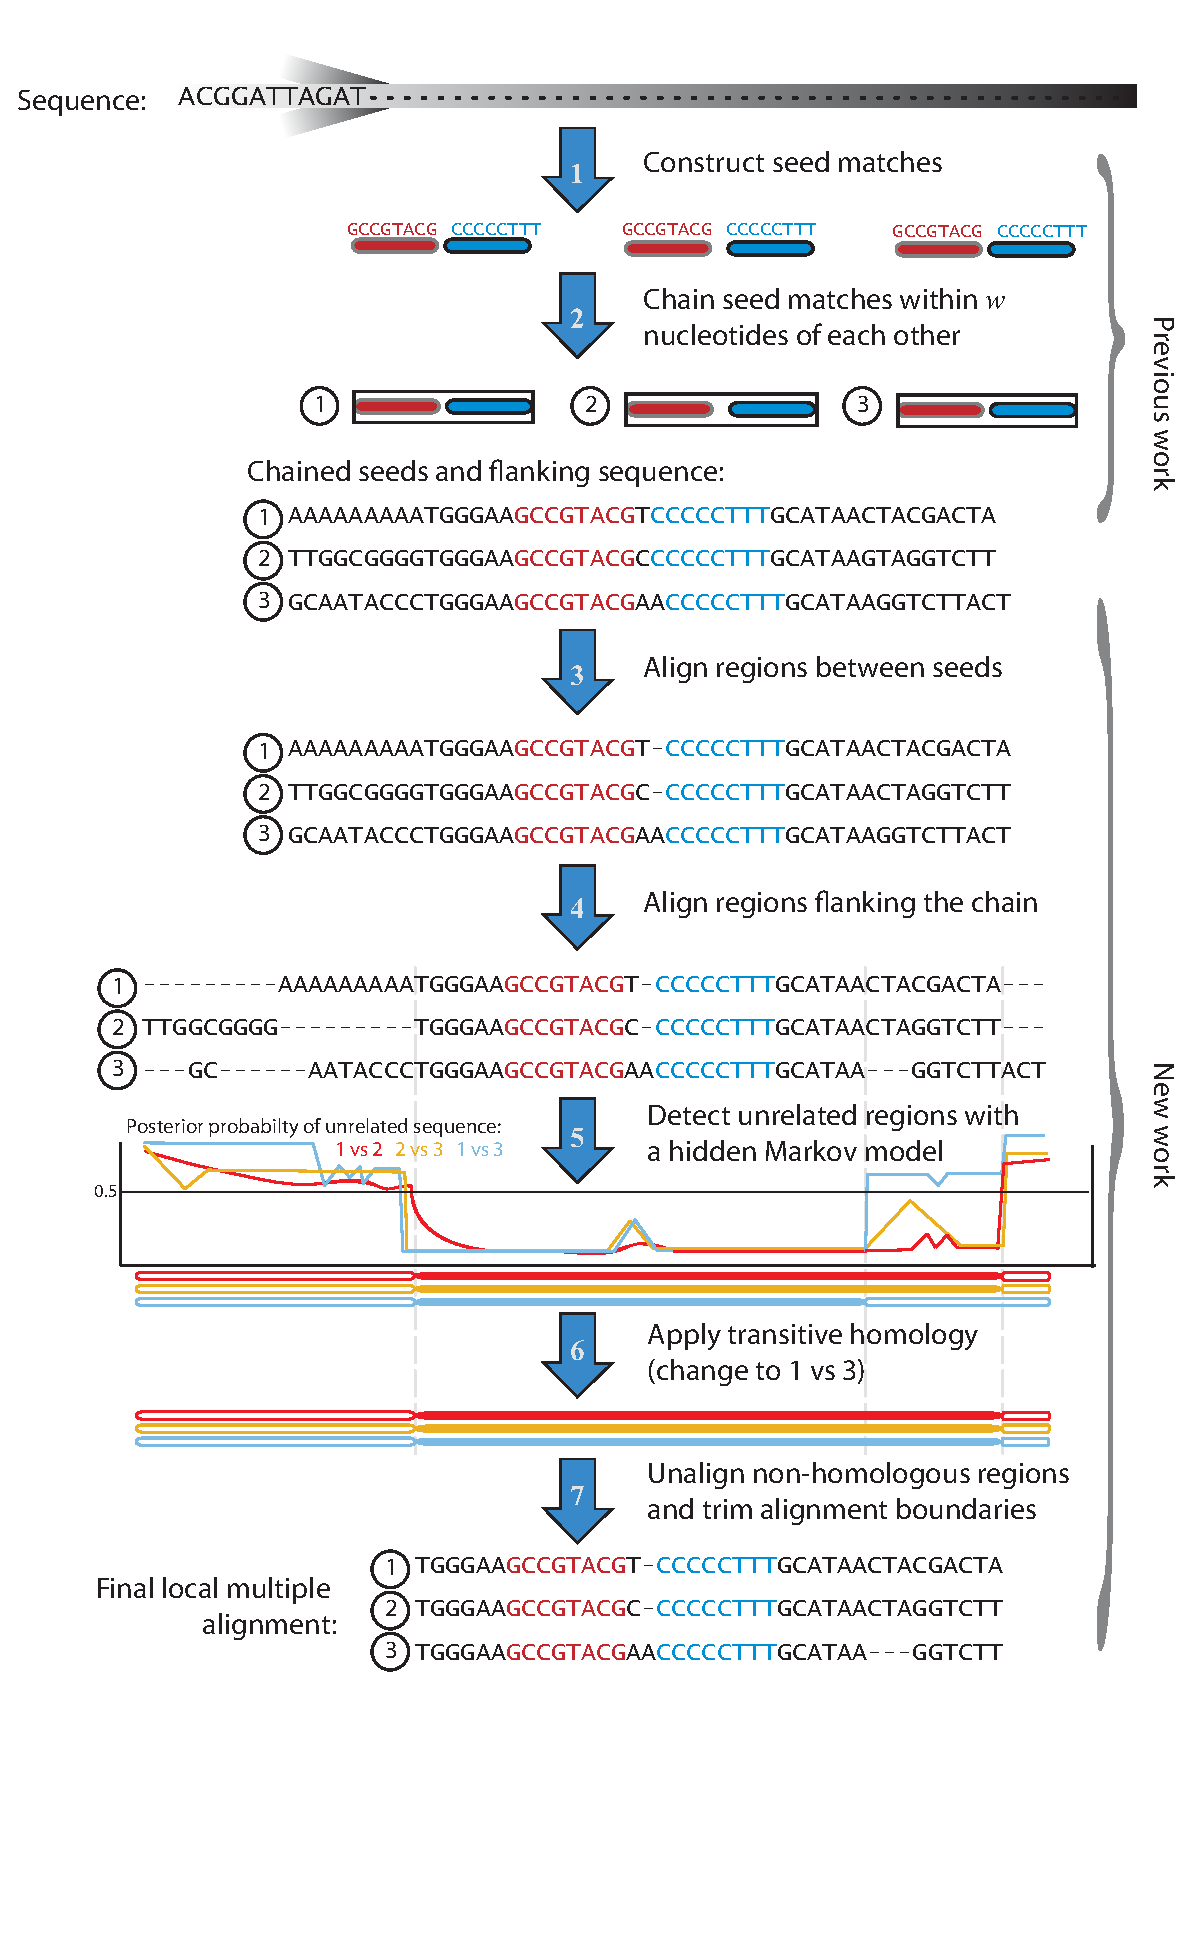
\epsfig{file=./figures/extension.eps,width=3.2in}}
\subfigure[Flowchart of the algorithmic process ]{ 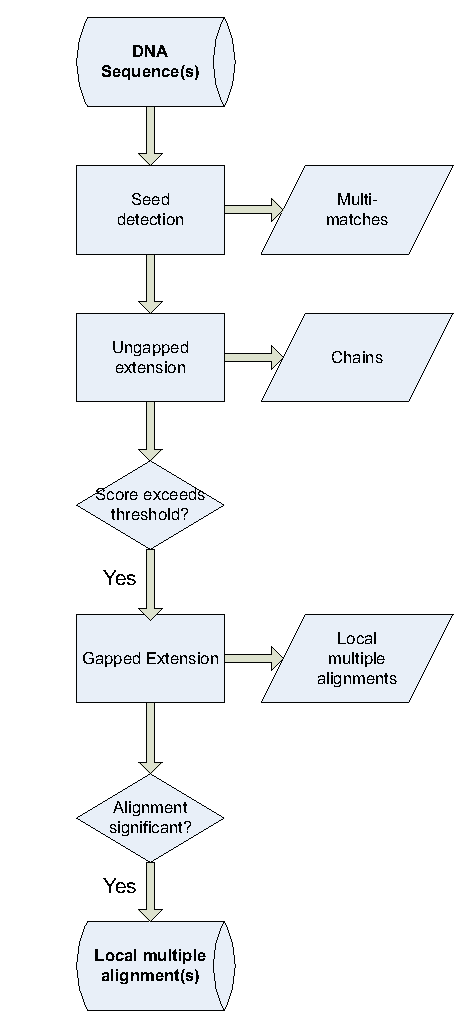
\epsfig{file=./figures/flowchart.eps,width=1.39in}}
\end{center}
\caption{Overview of the method, starting with an input sequence and ending with a set of local multiple alignments. First we (1) detect multi-matches in input sequence(s) using palindromic spaced seeds, then we perform (2)prioritized chaining of all multi-matches, next we induce (3) gapped extension of all high scoring chains. After gapped extension, we estimate the boundaries of homologous sequence using a random walk, and finally,(5) unalign any remaining non-homologous sequence using a pairwise homology test. }
\end{figure}


%\colorbox[named]{Gray}{adfa}

\subsection{Detecting seeds using a palindromic seed patterns}

As a starting point for homology detection, we locate all spaced seeds of a given weight $z$ in the input sequence(s). The palindromic spaced seed pattern is analyzed at each position in the input sequence to identify all multi-matches.  Previously we have demonstrated that palindromic spaced seeds offer good efficiency and sensitivity on a variety of input sequences~\cite{ref-procrast}. 

\subsection{Creating chains of multi-matches}

Once we have generated a list of multi-matches, we rely on our previously described method for efficiently filtration method for chaining ~\cite{ref-procrast}. A brief review of the method follows(for additional details refer to the manuscript).

In order to chain over each region of sequence $\mathcal{O}(1)$ times,
our method chains matches in order of decreasing multiplicity--we
extend the highest multiplicity matches first. When a match can no
longer be chained without including a gap larger than $w$
characters, our method identifies the neighboring \textit{subset}
matches within $w$ characters, i.e. the light gray seed in
Figure~\ref{fig:simple_extension}. We then \textit{link} each
neighboring subset match to the chained match. We refer to the
chained match as a \textit{superset} match. Rather than immediately
extend the subset match(es), we \textit{procrastinate} and extend
the subset match later when it has the highest multiplicity of any
match waiting to be extended. When chaining a match with a linked
superset (light gray in Figure~\ref{fig:simple_extension}), we
immediately include the entire region covered by the linked superset
match--obviating the need to re-examine sequence already covered by
a previous match extension.

Once we have finished the chaining process, we would like to score and evaluate the chained multi-matches to make a decision whether its worth spending computational resources on gapped extension. This idea has been used in other local multiple alignment heuristics~\cite{...} in order to minimize the number of gapped extensions that do not improve the boundaries of the chain.

\subsection{Gapped extension of high scoring chains}

Now that we have decided to performed a gapped extension in the current direction, we use MUSCLE to align the left/right region immediately surrounding the chains. The size of the extension window we send to MUSCLE is the lesser of 4*w or 200 nucleotides. The reasoning by setting our minimum extension window to 200nt is closely related to how we determine homology borders. Since we will assume that the extension window we have decided to align with MUSCLE is homologous over its entire length, we use random walk statistics to correct our assumption.

We start the random walk process by generating the path by scoring each column resulting gapped alignment via sum of pairs, using an inverted substitution matrix that rewards substitutions and indels, and penalizes matching nucleotides. Once generated, we start at our ladder point and take a step, 1nt at a time, to the left/right and keep track of the cumulative column score of our current position. We keep walking until we reach a cumulative score which is equal to our previously determined homology threshold(2727?). The idea is that, based on simulation data, this score represents a start of non-homologous sequence. FIXME!


Gapped extension in the current directions not yet finished as we need to make sure we are not classifying non-homologous DNA positions as homologous in our extended chains.

INSERT DETAILS ABOUT UNALIGNING NON-HOMOLOGOUS SEQUENCE HERE!


If have reached the end of the extension window without going beyond our homology threshold, we then improve our original seed boundaries and then trigger another round of chaining(and consequently another round of extension) in the same direction on the currently active, extend match. Else, if we surpass the homology threshold we first determine if our chain boundaries have been improved, and then signal that we are done chaining/extending the current match in the current direction. If we have already processed the current chain in both directions, we stop entirely and proceed to the next multi-match in the priority queue.

\subsubsection{Processing Novel homologous sequence}
Its worth mentioning that novel homologous sequence can be found during gapped extension.
FIXME: should briefly describe what we do with this!


Ideally, once our algorithm finishes we will have a complete listing of all homologous local mulitple alignments. This list could be potentially overwhelming, and even at this point, we still need a way of selecting only the highly significant alignments. 


\section{Results}
We have created a program called \texttt{procrastAligner} for Linux,
Windows, and Mac OS X that implements the described algorithm. Our
open-source implementation is available as C++ source code licensed
under the GPL.

\begin{figure}[t]
\scriptsize
\begin{verbatim}
GGGAGGATTGCTTGAACCTG--------GAGATTCAAGTGAGCTGAGATTGCACCACTGCATTCCAGCCTGGGC--AACAAAGCAAGACTCT-
AGGAGAATTGCTTGAACCTGGGAG-GCGGAGGTTGCAGTGAGCCGAGATGACGCCACTGCACTCCAGCCTGGGC--GACAGAGCA--------
AGGAGAATCGCTTGAACCCAAGAGAGTGAAGGTTGCAGTGAGCTGAGATCATGCCACTTCACTCCAGCCTGAGTGAAACAGC-----------
AGGAGAATAACTTCAACCTGGGAG-ACAGAGGTTGCAGTCAGCTGAGATCGCACCACTGCATTCCAGCCTGGGT--GACAGACCGAGACTCTG
AGGAGAACTGCTTGAACTCGGGAG-GCAGAGATTGCAGTGAGCTGAGATCATGTCAATGCACTGCAGCTTGAGT--GACAGAGTG--------
AGGAGAATCGCTTGAACCTGGGAG-GCAGAGGTTACAGAGAGCTGGGATTGTGCCACTGCACTCCGGCCTGGGC--AACAGAATG--------
A-CAGAATCACTTGAACCTGGGAG-GCAGAGGTTACAGTGAGCCAAAATCGCGCCACTGCACTCCAACCTGGGC--AACACAGCAA-------
AGGAGAATTGCTTGAACCCGGGAG-GTGGAGGCTGCAGTGAGCCGAGATCATGCCACTGCACTCCAGCCT-GGT--GACAGAGCGAGA-----
AGGAGAATTGTTTGAACCCAGGAG-GCGGAGGCTGCAGTGAGCCGAGATTGTGTCACTGTACTCCAGCCTGGGCAAGACAGAG----------
AGGAGAATCCCTTCAACCTGGGAA-ACAGAGGTTGCAGTGAGCCAAGATCGCACCATTGCACTCCAGTCTGGGC--AACAGAGAGA-------
*  ** *    ** ***           ***  *   * ****    **     **  * * * *    *  *      *

\end{verbatim}
\vspace{-0.5cm}
\normalsize
\caption{Partial alignment of Alu-Sc subfamily found in \emph{H. sapiens} C1 esterase inhibitor gene. Each row represents an aligned ALU.}.
\end{figure}

\subsection{Comparison with RepeatScount}

RepeatScout generates a repeat family consensus for all high frequency kmers via ungapped extension. As output, RepeatScout returns all families atleast 50nt long and occuring atleast 3 times in the input sequence(s). Once finished, RepeatScout uses RepeatMasker to locate all occurences of the repeat family in the input sequence(s).

How can we compare this to procrastAligner? 


\section{Discussion}
\subsubsection{Comparison of gapped
extension approaches}


\begin{itemize}

\item RepeatScout extends one nucleotide at a time
\item ABA merges pairwise matches and resolves inconsistencies by
whorl and bulge removal
\item multiz? and HomologMiner? also merge pairwise matches, how do
they resolve inconsistency?
\item procrastAligner generates multiple alignments using libMUSCLE,
which does progressive multiple alignment.  Progressive means that
pairwise alignments do enter in at some stage, but for higher
multiplicity matches, much of the alignment is multiple alignment.
cite a paper which shows multiple alignment is more accurate than
pairwise alignment.  MUSCLE's iterative refinement procedure ensures
a high-scoring alignment irrespective of guide tree.

\end{itemize}


\subsection{Significance estimation and simulations}

Finally, we would like to extend blast statistics to multiple local alignment. How?
\begin{itemize}
\item Extending Repseek simulations to multiple
\item Tompa et al, estimating the parameters for multiple alignments
\item will involve running procrastAlign with fixed parameters on sequences varying in composition and length
\item also will have to take into account multiplicity
\item FIXME: fill in more details on Monday
\end{itemize}

\section{ Acknowledgments }
AED was supported by NLM Training Grant 5T15LM007359-05. TJT was
supported by Spanish Ministry MECD Grant TIN2004-03382 and AGAUR
Training Grant FI-IQUC-2005.

\bibliographystyle{splncs}
\small
\bibliography{procrastination}


\end{document}
